% Section content template for individual Educative lessons
% This file contains the actual content for a specific section
% Generated from Educative API section content

% Section: Focus on Client-Side Errors in a Monitoring System
% Section ID: 4768611427680256
% Section Slug: focus-on-client-side-errors-in-a-monitoring-system
% Generated: 2025-12-07T18:42:54.528527

\subsection{Client-side errors}\label{bKhd4NBIu0-aA3erZoS6y}
\\
In a distributed system, clients often access the service via an HTTP request. We can monitor our web and application servers' logs if a request fails to process. If multiple requests fail, we can observe a spike in internal errors (error 500).
\\
Those errors whose root cause is on the client side are hard to respond to because the service has little to no insight into the client's system. We might try to look for a dip in the load compared to averages, but such a graph is usually hard. It can have false positives and false negatives due to factors such as unexpectedly variable load or if a small portion of the client population is affected.
\\
There are many factors that can cause failures that can result in clients being unable to reach the server. These include the following:

\begin{itemize}
\item
\protect\phantomsection\label{Q5qDU9AfrVr9cI1fu10K2}
Failure in DNS name resolution.
\item
\protect\phantomsection\label{Hjqwnh3ggcLLbTTtU-EJt}
Any failure in routing along the path from the client to the service provider.
\item
\protect\phantomsection\label{yqG287Vxr_tdkgbQz5nAV}
Any failures with third-party infrastructure, such as middleboxes and content delivery networks (CDNs).
\end{itemize}

\begin{figure}[htbp]
 \centering
 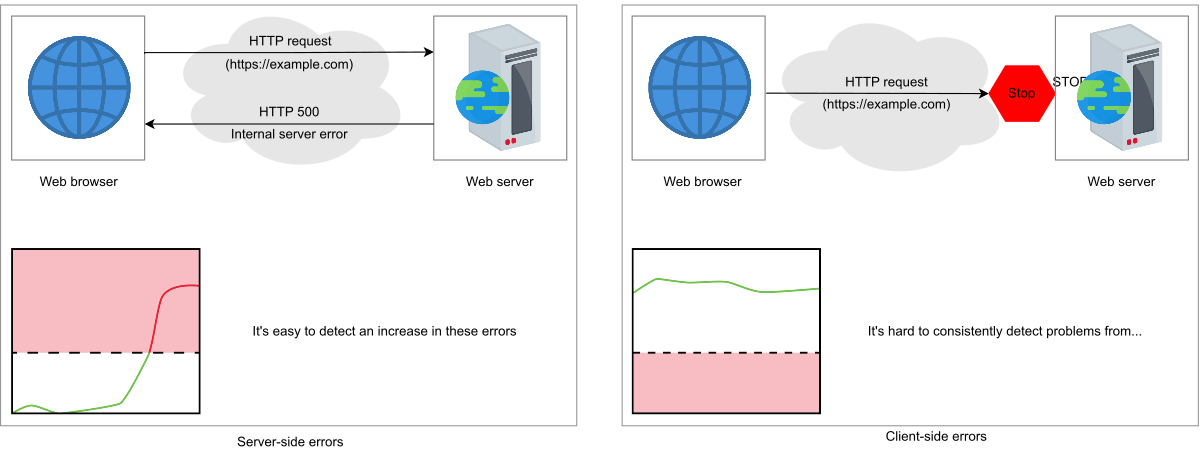
\includegraphics[width=0.5\textwidth]{Images/chapter_15/section_4768611427680256/4741252860084224.png}
 \caption{Server-side errors versus client-side errors}
\end{figure}

\subsection{Failures due to a routing bug}\label{iBE3sxtwaDFizGT_-4tl6}
\\
Let's look at a real-world example of an error that impacted a large number of service customers, but the service wasn't readily aware of it.
\\
One of Google's peer ISPs accidentally announced Internet routes that it wasn't supposed to. As a result, the traffic of many of Google's customers started routing through unintended ISPs and wasn't reaching Google because of the BGP leak; one of the examples of the BGP leak is shown in the illustration below. Clients were frustrated because they weren't able to reach Google, while Google might have been unaware of such problems right away because these issues didn't happen on its infrastructure.
\begin{quote}
We can learn more about this event by clicking here. BGP
\end{quote}

\begin{figure}[htbp]
 \centering
 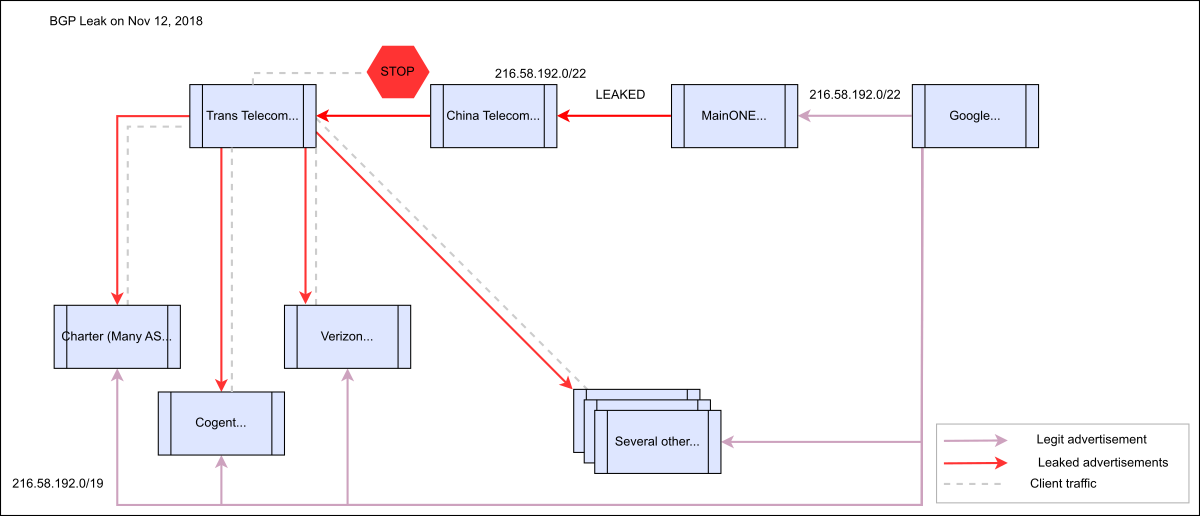
\includegraphics[width=0.5\textwidth]{Images/chapter_15/section_4768611427680256/5767472710680576.png}
 \caption{BGP leak}
\end{figure}

The above leak isn\textquotesingle t unique. Similar issues keep arising. Another such leakage happened on April 16, 2021, when an AS mistakenly announced over 30,000 BGP prefixes. This resulted in a 13 times spike in the inbound traffic to their network. However, an increase in influx was observed, and the problem was solved.\\
\strut \\
The impacted services\textquotesingle{} monitoring systems might not catch the above events readily.\\
Monitoring such situations is crucial so that the application remains available for all of its customers. Therefore, in the next lessons, we'll go through methods that help us to monitor the situations mentioned above.\\
\strut \\

% End of section content